%%%%%%%%%%%%%%%%%%%%%%%%%%%%%%%%%%%%%%%%%%%%%%%%%%%%%%%%%%%%%%%
%
% Welcome to Overleaf --- just edit your LaTeX on the left,
% and we'll compile it for you on the right. If you give
% someone the link to this page, they can edit at the same
% time. See the help menu above for more info. Enjoy!
%
% Note: you can export the pdf to see the result at full
% resolution.
%
%%%%%%%%%%%%%%%%%%%%%%%%%%%%%%%%%%%%%%%%%%%%%%%%%%%%%%%%%%%%%%%
% Mindmap
% Author: Stefan Kottwitz
% https://www.packtpub.com/hardware-and-creative/latex-cookbook
\documentclass[border = 60pt]{standalone} 
%%%<
\usepackage{verbatim}
%%%>
\begin{comment}
:Title: Mindmap
:Tags: Mindmaps;Cookbook
:Author: Stefan Kottwitz
:Slug: mindmap

A mindmap of TeX concepts.
\end{comment}
% \usepackage[landscape]{geometry}
\usepackage{tikz}
\usetikzlibrary{mindmap}
% \usepackage{metalogo}
% \usepackage{dtklogos}

\definecolor{fond}{rgb}{0,0.41,0.54} % dark blue

\begin{document}
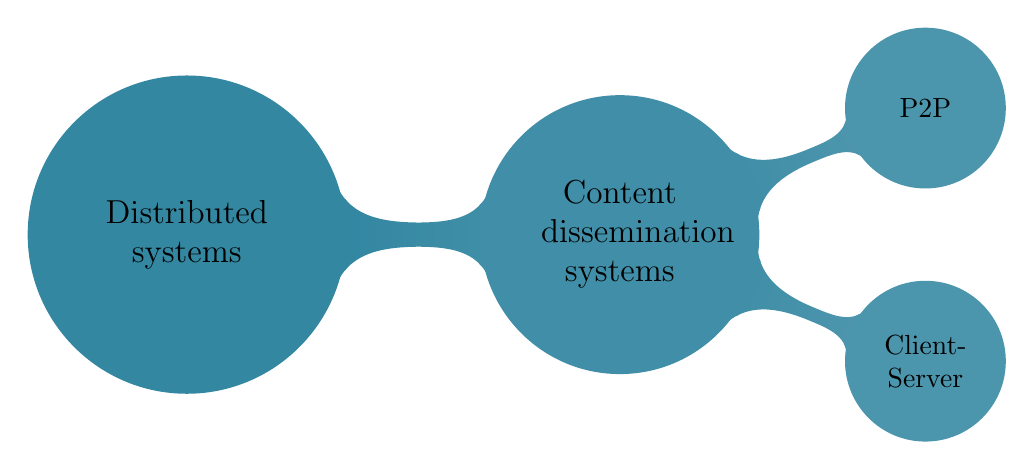
\begin{tikzpicture}[
    mindmap,
    text = black,
    every node/.style=concept,
    concept color=fond!80!white,
    grow cyclic,
    level 1/.append style={font=\large, minimum size=3.5cm, level distance=5.5cm, sibling angle=90},
    level 2/.append style={font=\normalsize, minimum size=2cm, level distance=4.2cm,sibling angle=45},
    level 3/.append style={font=\normalsize, minimum size=1.6cm, level distance=3cm,sibling angle=45}
    ]
    
   \node [root concept] {Distributed systems}
      child [concept color=fond!75!white] { node {Content\\ dissemination systems}
         child [concept color=fond!70!white] {node {Client-Server}}
         child [concept color=fond!70!white] {node {P2P}
%             child[concept color=fond!15!red!60!white] {node {Gossip}}
%             child[concept color=fond!60!white] {node {Mesh}}
%             child[concept color=fond!60!white] {node {Tree}}
            }
         };
\end{tikzpicture}
\end{document}
% 
% \begin{document}
% \begin{tikzpicture}
%   \path [
%     mindmap,
%     text = white,
%     grow cyclic,
%     level 1 concept/.append style = {font=\Large\bfseries, sibling angle=90},
%     level 2 concept/.append style = {font=\normalsize\bfseries},
%     level 3 concept/.append style = {font=\small\bfseries},
%     tex/.style     = {concept, ball color=blue, font=\Huge\bfseries},
%     engines/.style = {concept, ball color=green!50!black},
%     formats/.style = {concept, ball color=blue!50!black},
% %     systems/.style = {concept, ball color=red!90!black},
%     systems/.style = {concept, ball color=blue!30},
%     editors/.style = {concept, ball color=orange!90!black}
%   ]
%   node [tex, grow=100] {Content dissemination} [clockwise from=315]
%     child [concept color=blue!80!black, nodes={engines}] {
%       node {P2P} [clockwise from=330]
%         child[text=black, concept color=blue!40!black, nodes={systems}] { node {Gossip} }
%         child[concept color=blue!40!black, nodes={systems}] { node {Trees} }
%         child[concept color=blue!40!black, nodes={systems}] { node {Meshes}}}
%     child [concept color=green, nodes={engines}] {
%       node {Client-Server} [clockwise from=330]
%     };
%     %child [concept color=red, nodes={systems}] {
%     %  node {Systems} [clockwise from=210]
%     %    child { node {\TeX Live} [clockwise from=300]
%     %      child { node {Mac \TeX} }}
%     %    child { node {MiK\TeX} [clockwise from=60]
%     %      child { node {Pro \TeX t} }}}
%     %child [concept color=orange, nodes={editors}] {
%     %  node {Editors} };
% \end{tikzpicture}
% \end{document}